\documentclass[
]{jss}

\usepackage[utf8]{inputenc}

\providecommand{\tightlist}{%
  \setlength{\itemsep}{0pt}\setlength{\parskip}{0pt}}

\author{
FirstName LastName\\University/Company \And Second Author\\Affiliation
}
\title{Text analysis of Trump's tweets \pkg{foo}}

\Plainauthor{FirstName LastName, Second Author}
\Plaintitle{Text analysis of Trump's tweets}
\Shorttitle{\pkg{foo}: Text analysis}

\Abstract{
The abstract of the article.
}

\Keywords{keywords, not capitalized, \proglang{Java}}
\Plainkeywords{keywords, not capitalized, Java}

%% publication information
%% \Volume{50}
%% \Issue{9}
%% \Month{June}
%% \Year{2012}
%% \Submitdate{}
%% \Acceptdate{2012-06-04}

\Address{
    FirstName LastName\\
  University/Company\\
  First line Second line\\
  E-mail: \email{name@company.com}\\
  URL: \url{http://rstudio.com}\\~\\
    }


% Pandoc header

\usepackage{amsmath}

\begin{document}

When Trump wishes the Olympic team good luck, he's tweeting from his
iPhone. When he's insulting a rival, he's usually tweeting from an
Android. Is this an artifact showing which tweets are Trump's own and
which are by some handler?

Others have
\href{http://www.cnet.com/news/trumps-tweets-android-for-nasty-iphone-for-nice/}{explored
Trump's timeline} and noticed this tends to hold up- and Trump himself
\href{http://www.theverge.com/2015/10/5/9453935/donald-trump-twitter-strategy}{does
indeed tweet from a Samsung Galaxy}. But how could we examine it
quantitatively? I've been writing about text mining and
\href{http://varianceexplained.org/r/yelp-sentiment/}{sentiment
analysis} recently, particularly during my development of the
\href{http://github.com/juliasilge/tidytext}{tidytext R package} with
Julia Silge, and this is a great opportunity to apply it again.

My analysis, shown below, concludes that \textbf{the Android and iPhone
tweets are clearly from different people}, posting during different
times of day and using hashtags, links, and retweets in distinct ways.
What's more, we can see that \textbf{the Android tweets are angrier and
more negative}, while the iPhone tweets tend to be benign announcements
and pictures. Overall I'd agree with
\citep{tvaziri}(\url{https://twitter.com/tvaziri})'s analysis: this lets
us tell the difference between the campaign's tweets (iPhone) and
Trump's own (Android).

\hypertarget{the-dataset}{%
\subsubsection{The dataset}\label{the-dataset}}

First we'll retrieve the content of Donald Trump's timeline using the
\texttt{userTimeline} function in the
\href{https://cran.r-project.org/web/packages/twitteR}{twitteR}
package:\footnote{To keep the post concise I don't show all of the code,
  especially code that generates figures. But you can find the full code
  \href{https://github.com/dgrtwo/dgrtwo.github.com/blob/master/_R/2016-08-09-trump-tweets.Rmd}{here}.}

\begin{CodeChunk}

\begin{CodeInput}
R> library(dplyr)
\end{CodeInput}

\begin{CodeOutput}

Attaching package: 'dplyr'
\end{CodeOutput}

\begin{CodeOutput}
The following objects are masked from 'package:stats':

    filter, lag
\end{CodeOutput}

\begin{CodeOutput}
The following objects are masked from 'package:base':

    intersect, setdiff, setequal, union
\end{CodeOutput}

\begin{CodeInput}
R> library(purrr)
R> library(ggplot2)
R> library(twitteR)
\end{CodeInput}

\begin{CodeOutput}

Attaching package: 'twitteR'
\end{CodeOutput}

\begin{CodeOutput}
The following objects are masked from 'package:dplyr':

    id, location
\end{CodeOutput}
\end{CodeChunk}

\begin{CodeChunk}

\begin{CodeInput}
R> # if you want to follow along without setting up Twitter authentication,
R> # just use my dataset:
R> load(url("http://varianceexplained.org/files/trump_tweets_df.rda"))
\end{CodeInput}
\end{CodeChunk}

We clean this data a bit, extracting the source application. (We're
looking only at the iPhone and Android tweets- a much smaller number are
from the web client or iPad).

\begin{CodeChunk}

\begin{CodeInput}
R> library(tidyr)
R> 
R> tweets <- trump_tweets_df %>%
R+   select(id, statusSource, text, created) %>%
R+   extract(statusSource, "source", "Twitter for (.*?)<") %>%
R+   filter(source %in% c("iPhone", "Android"))
\end{CodeInput}
\end{CodeChunk}

Overall, this includes 628 tweets from iPhone, and 762 tweets from
Android.

One consideration is what time of day the tweets occur, which we'd
expect to be a ``signature'' of their user. Here we can certainly spot a
difference:

\begin{CodeChunk}

\begin{CodeInput}
R> library(lubridate)
\end{CodeInput}

\begin{CodeOutput}

Attaching package: 'lubridate'
\end{CodeOutput}

\begin{CodeOutput}
The following objects are masked from 'package:dplyr':

    intersect, setdiff, union
\end{CodeOutput}

\begin{CodeOutput}
The following objects are masked from 'package:base':

    date, intersect, setdiff, union
\end{CodeOutput}

\begin{CodeInput}
R> library(scales)
\end{CodeInput}

\begin{CodeOutput}

Attaching package: 'scales'
\end{CodeOutput}

\begin{CodeOutput}
The following object is masked from 'package:purrr':

    discard
\end{CodeOutput}

\begin{CodeInput}
R> tweets %>%
R+   count(source, hour = hour(with_tz(created, "EST"))) %>%
R+   mutate(percent = n / sum(n)) %>%
R+   ggplot(aes(hour, percent, color = source)) +
R+   geom_line() +
R+   scale_y_continuous(labels = percent_format()) +
R+   labs(x = "Hour of day (EST)",
R+        y = "% of tweets",
R+        color = "")
\end{CodeInput}


\begin{center}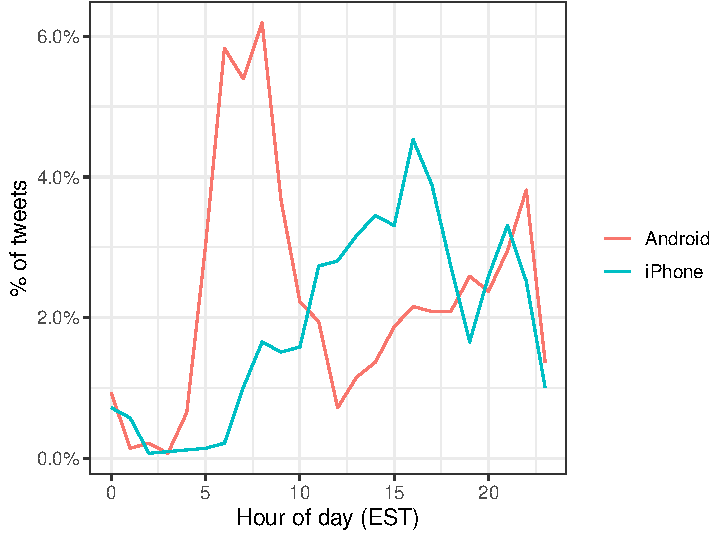
\includegraphics{Live_Demo2_files/figure-latex/unnamed-chunk-2-1} \end{center}

\end{CodeChunk}

Trump on the Android does a lot more tweeting in the morning, while the
campaign posts from the iPhone more in the afternoon and early evening.

Another place we can spot a difference is in Trump's anachronistic
behavior of ``manually retweeting'' people by copy-pasting their tweets,
then surrounding them with quotation marks:

Almost all of these quoted tweets are posted from the Android:

\begin{CodeChunk}


\begin{center}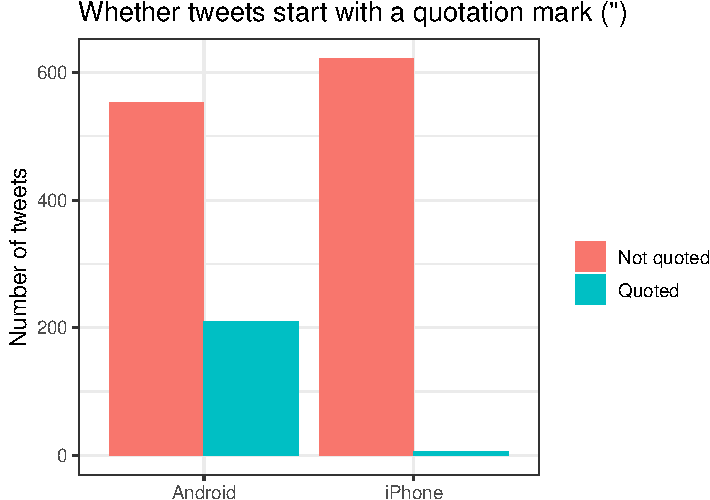
\includegraphics{Live_Demo2_files/figure-latex/unnamed-chunk-3-1} \end{center}

\end{CodeChunk}

In the remaining by-word analyses in this text, I'll filter these quoted
tweets out (since they contain text from followers that may not be
representative of Trump's own tweets).

Somewhere else we can see a difference involves sharing links or
pictures in tweets.

\begin{CodeChunk}

\begin{CodeInput}
R> tweet_picture_counts <- tweets %>%
R+   filter(!str_detect(text, '^"')) %>%
R+   count(source,
R+         picture = ifelse(str_detect(text, "t.co"),
R+                          "Picture/link", "No picture/link"))
R> 
R> ggplot(tweet_picture_counts, aes(source, n, fill = picture)) +
R+   geom_bar(stat = "identity", position = "dodge") +
R+   labs(x = "", y = "Number of tweets", fill = "")
\end{CodeInput}


\begin{center}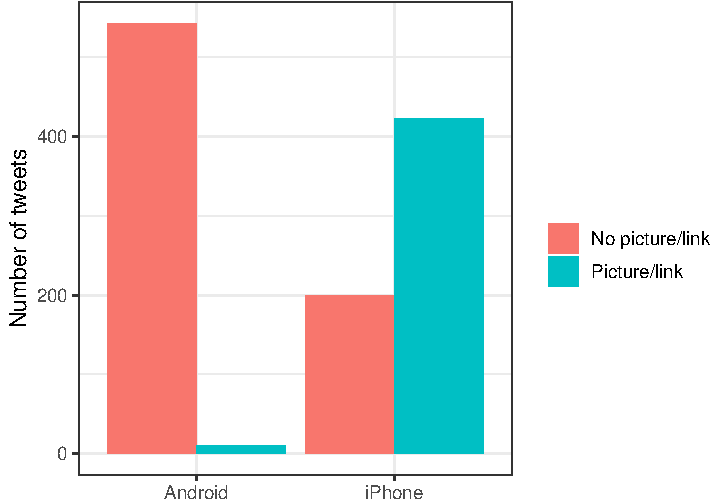
\includegraphics{Live_Demo2_files/figure-latex/unnamed-chunk-4-1} \end{center}

\end{CodeChunk}

\begin{CodeChunk}

\begin{CodeOutput}
Warning: funs() is soft deprecated as of dplyr 0.8.0
Please use a list of either functions or lambdas: 

  # Simple named list: 
  list(mean = mean, median = median)

  # Auto named with `tibble::lst()`: 
  tibble::lst(mean, median)

  # Using lambdas
  list(~ mean(., trim = .2), ~ median(., na.rm = TRUE))
This warning is displayed once per session.
\end{CodeOutput}
\end{CodeChunk}

It turns out tweets from the iPhone were \textbf{38 times as likely to
contain either a picture or a link.} This also makes sense with our
narrative: the iPhone (presumably run by the campaign) tends to write
``announcement'' tweets about events, like this:

\hypertarget{comparison-of-words}{%
\subsubsection{Comparison of words}\label{comparison-of-words}}

Now that we're sure there's a difference between these two accounts,
what can we say about the difference in the \emph{content}? We'll use
the \href{https://cran.r-project.org/web/packages/tidytext}{tidytext}
package that \href{http://juliasilge.com/}{Julia Silge} and I developed.

We start by dividing into individual words using the
\texttt{unnest\_tokens} function (see
\href{https://cran.r-project.org/web/packages/tidytext/vignettes/tidytext.html}{this
vignette} for more), and removing some common ``stopwords''\footnote{We
  had to use a custom regular expression for Twitter, since typical
  tokenizers would split the \# off of hashtags and @ off of usernames.
  We also removed links and ampersands (\texttt{\&amp;}) from the text.}:

\begin{CodeChunk}

\begin{CodeInput}
R> library(tidytext)
R> 
R> reg <- "([^A-Za-z\\d#@']|'(?![A-Za-z\\d#@]))"
R> tweet_words <- tweets %>%
R+   filter(!str_detect(text, '^"')) %>%
R+   mutate(text = str_replace_all(text, "https://t.co/[A-Za-z\\d]+|&amp;", "")) %>%
R+   unnest_tokens(word, text, token = "regex", pattern = reg) %>%
R+   filter(!word %in% stop_words$word,
R+          str_detect(word, "[a-z]"))
R> 
R> tweet_words
\end{CodeInput}

\begin{CodeOutput}
# A tibble: 8,753 x 4
   id                 source created             word                  
   <chr>              <chr>  <dttm>              <chr>                 
 1 676494179216805888 iPhone 2015-12-14 20:09:15 record                
 2 676494179216805888 iPhone 2015-12-14 20:09:15 health                
 3 676494179216805888 iPhone 2015-12-14 20:09:15 #makeamericagreatagain
 4 676494179216805888 iPhone 2015-12-14 20:09:15 #trump2016            
 5 676509769562251264 iPhone 2015-12-14 21:11:12 accolade              
 6 676509769562251264 iPhone 2015-12-14 21:11:12 @trumpgolf            
 7 676509769562251264 iPhone 2015-12-14 21:11:12 highly                
 8 676509769562251264 iPhone 2015-12-14 21:11:12 respected             
 9 676509769562251264 iPhone 2015-12-14 21:11:12 golf                  
10 676509769562251264 iPhone 2015-12-14 21:11:12 odyssey               
# ... with 8,743 more rows
\end{CodeOutput}
\end{CodeChunk}

What were the most common words in Trump's tweets overall?

\begin{CodeChunk}


\begin{center}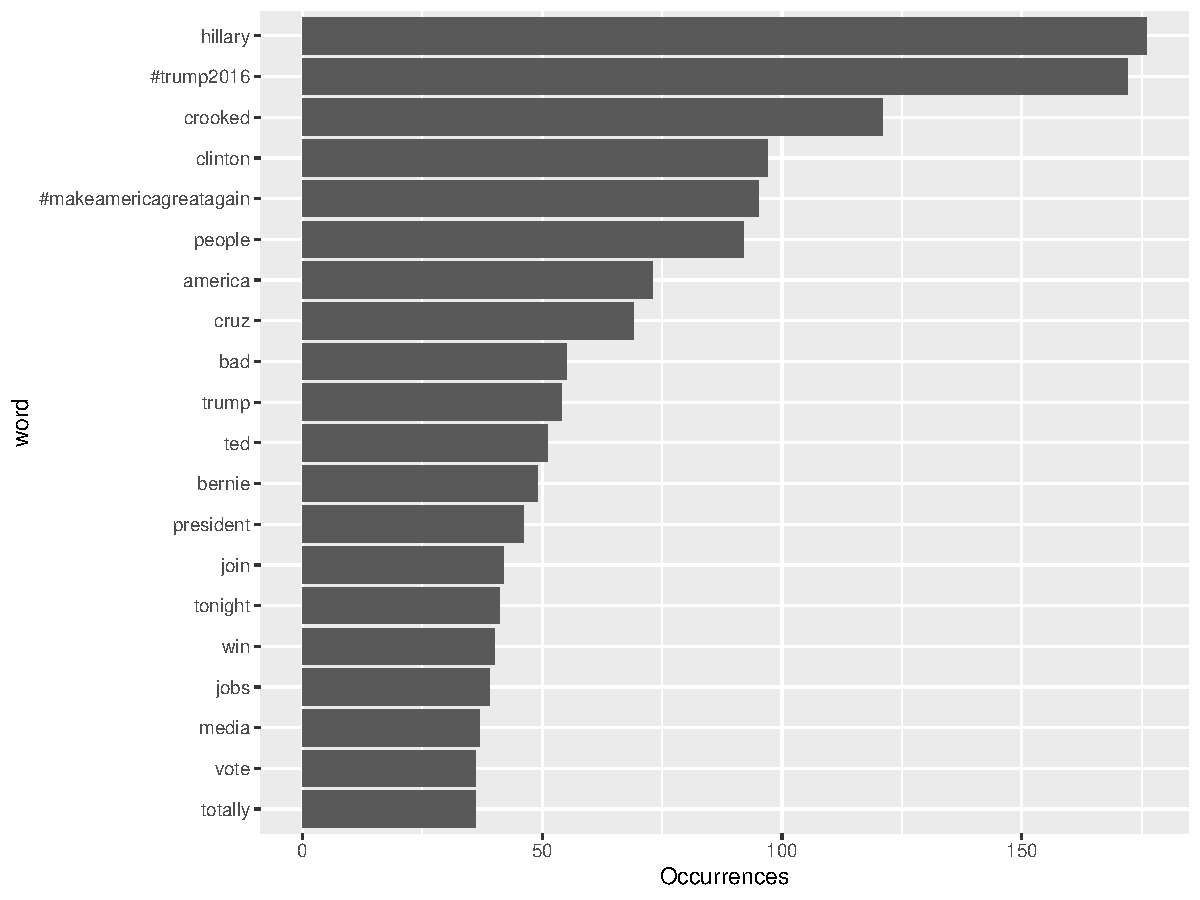
\includegraphics{Live_Demo2_files/figure-latex/tweet_words_plot-1} \end{center}

\end{CodeChunk}

These should look familiar for anyone who has seen the feed. Now let's
consider which words are most common from the Android relative to the
iPhone, and vice versa. We'll use the simple measure of log odds ratio,
calculated for each word as:\footnote{The ``plus ones,'' called
  \href{https://en.wikipedia.org/wiki/Additive_smoothing}{Laplace
  smoothing} are to avoid dividing by zero and to put
  \href{http://varianceexplained.org/r/empirical_bayes_baseball/}{more
  trust in common words}.}

\[\log_2(\frac{\frac{\mbox{\#\ in Android} + 1}{\mbox{Total Android} + 1}}
  {\frac{\mbox{\#\ in iPhone} + 1}{\mbox{Total iPhone} + 1}})\]

\begin{CodeChunk}

\begin{CodeInput}
R> android_iphone_ratios <- tweet_words %>%
R+   count(word, source) %>%
R+   filter(sum(n) >= 5) %>%
R+   spread(source, n, fill = 0) %>%
R+   ungroup() %>%
R+   mutate_each(funs((. + 1) / sum(. + 1)), -word) %>%
R+   mutate(logratio = log2(Android / iPhone)) %>%
R+   arrange(desc(logratio))
\end{CodeInput}
\end{CodeChunk}

Which are the words most likely to be from Android and most likely from
iPhone?

\begin{CodeChunk}


\begin{center}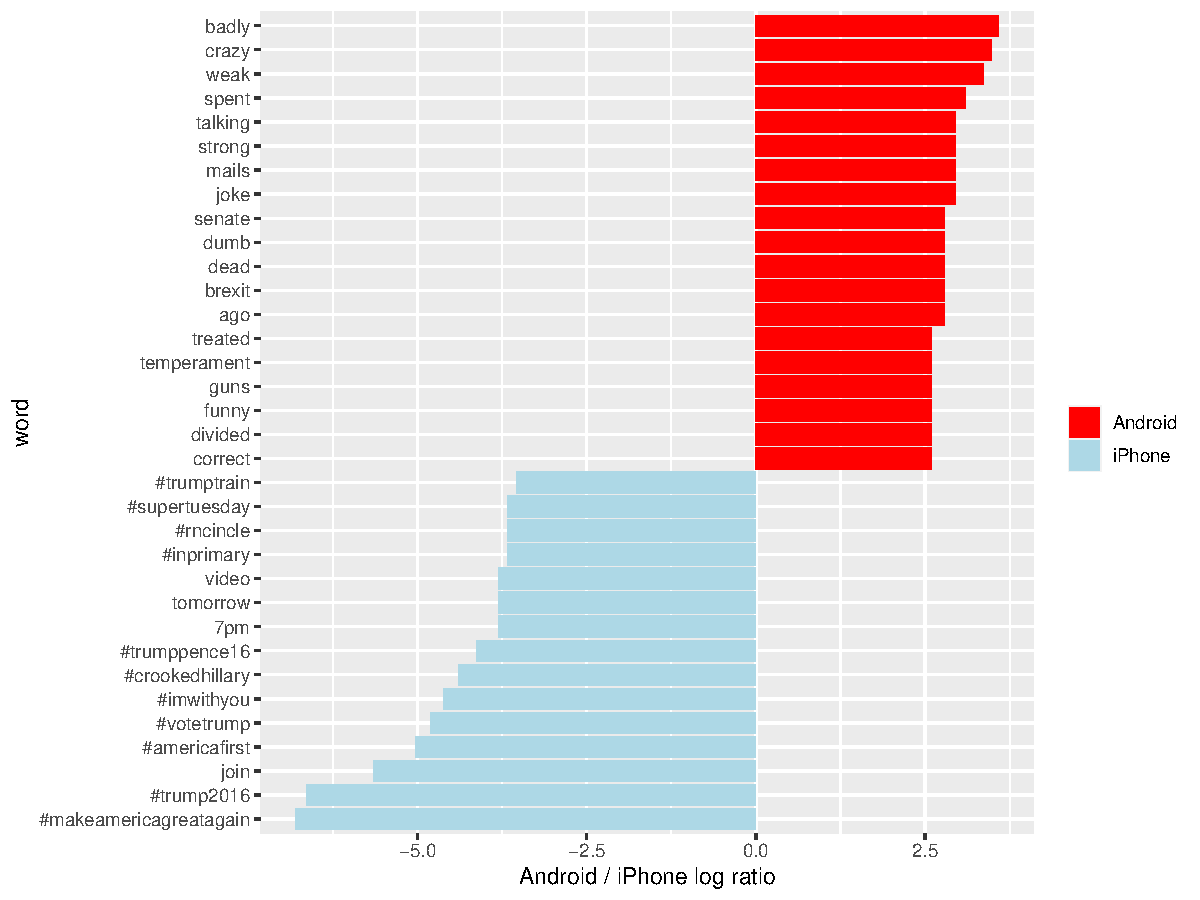
\includegraphics{Live_Demo2_files/figure-latex/android_iphone_ratios_plot-1} \end{center}

\end{CodeChunk}

A few observations:

\begin{itemize}
\item
  \textbf{Most hashtags come from the iPhone}. Indeed, almost no tweets
  from Trump's Android contained hashtags, with some rare exceptions
  like
  \href{https://twitter.com/realDonaldTrump/status/753960134422900736}{this
  one}. (This is true only because we filtered out the quoted
  ``retweets'', as Trump does sometimes quote tweets
  \href{https://twitter.com/realDonaldTrump/status/731805331425218560}{like
  this} that contain hashtags).
\item
  \textbf{Words like ``join'' and ``tomorrow'', and times like ``7pm'',
  also came only from the iPhone}. The iPhone is clearly responsible for
  event announcements like
  \href{https://twitter.com/realDonaldTrump/status/743522630230228993}{this
  one} (``Join me in Houston, Texas tomorrow night at 7pm!'')
\item
  \textbf{A lot of ``emotionally charged'' words, like ``badly'',
  ``crazy'', ``weak'', and ``dumb'', were overwhelmingly more common on
  Android.} This supports the original hypothesis that this is the
  ``angrier'' or more hyperbolic account.
\end{itemize}

\hypertarget{sentiment-analysis-trumps-tweets-are-much-more-negative-than-his-campaigns}{%
\subsubsection{Sentiment analysis: Trump's tweets are much more negative
than his
campaign's}\label{sentiment-analysis-trumps-tweets-are-much-more-negative-than-his-campaigns}}

Since we've observed a difference in sentiment between the Android and
iPhone tweets, let's try quantifying it. We'll work with the
\href{http://saifmohammad.com/WebPages/NRC-Emotion-Lexicon.htm}{NRC
Word-Emotion Association} lexicon, available from the tidytext package,
which associates words with 10 sentiments: \textbf{positive},
\textbf{negative}, \textbf{anger}, \textbf{anticipation},
\textbf{disgust}, \textbf{fear}, \textbf{joy}, \textbf{sadness},
\textbf{surprise}, and \textbf{trust}.

\begin{CodeChunk}

\begin{CodeInput}
R> library(tidytext)
R> library(textdata)
R> nrc <- get_sentiments("nrc")
\end{CodeInput}
\end{CodeChunk}

To measure the sentiment of the Android and iPhone tweets, we can count
the number of words in each category:

\begin{CodeChunk}

\begin{CodeInput}
R> sources <- tweet_words %>%
R+   group_by(source) %>%
R+   mutate(total_words = n()) %>%
R+   ungroup() %>%
R+   distinct(id, source, total_words)
R> 
R> by_source_sentiment <- tweet_words %>%
R+   inner_join(nrc, by = "word") %>%
R+   count(sentiment, id) %>%
R+   ungroup() %>%
R+   complete(sentiment, id, fill = list(n = 0)) %>%
R+   inner_join(sources) %>%
R+   group_by(source, sentiment, total_words) %>%
R+   summarize(words = sum(n)) %>%
R+   ungroup()
\end{CodeInput}

\begin{CodeOutput}
Joining, by = "id"
\end{CodeOutput}

\begin{CodeInput}
R> head(by_source_sentiment)
\end{CodeInput}

\begin{CodeOutput}
# A tibble: 6 x 4
  source  sentiment    total_words words
  <chr>   <chr>              <int> <dbl>
1 Android anger               4901   321
2 Android anticipation        4901   256
3 Android disgust             4901   207
4 Android fear                4901   268
5 Android joy                 4901   199
6 Android negative            4901   560
\end{CodeOutput}
\end{CodeChunk}

(For example, we see that 321 of the 4901 words in the Android tweets
were associated with ``anger''). We then want to measure how much more
likely the Android account is to use an emotionally-charged term
relative to the iPhone account. Since this is count data, we can use a
\href{https://stat.ethz.ch/R-manual/R-devel/library/stats/html/poisson.test.html}{Poisson
test} to measure the difference:

\begin{CodeChunk}

\begin{CodeInput}
R> library(broom)
R> 
R> sentiment_differences <- by_source_sentiment %>%
R+   group_by(sentiment) %>%
R+   do(tidy(poisson.test(.$words, .$total_words)))
R> 
R> sentiment_differences
\end{CodeInput}

\begin{CodeOutput}
# A tibble: 10 x 9
# Groups:   sentiment [10]
   sentiment estimate statistic  p.value parameter conf.low conf.high method
   <chr>        <dbl>     <dbl>    <dbl>     <dbl>    <dbl>     <dbl> <chr> 
 1 anger         1.49       321 2.19e- 5      274.    1.24       1.81 Compa~
 2 anticipa~     1.17       256 1.19e- 1      240.    0.960      1.43 Compa~
 3 disgust       1.68       207 1.78e- 5      170.    1.31       2.16 Compa~
 4 fear          1.56       268 1.89e- 5      226.    1.26       1.93 Compa~
 5 joy           1.00       199 1.00e+ 0      199.    0.809      1.24 Compa~
 6 negative      1.69       560 7.09e-13      459.    1.46       1.97 Compa~
 7 positive      1.06       555 3.82e- 1      541.    0.930      1.21 Compa~
 8 sadness       1.62       303 1.15e- 6      252.    1.33       1.99 Compa~
 9 surprise      1.17       159 2.17e- 1      149.    0.908      1.51 Compa~
10 trust         1.13       369 1.47e- 1      351.    0.960      1.33 Compa~
# ... with 1 more variable: alternative <chr>
\end{CodeOutput}
\end{CodeChunk}

And we can visualize it with a 95\% confidence interval:

\begin{CodeChunk}


\begin{center}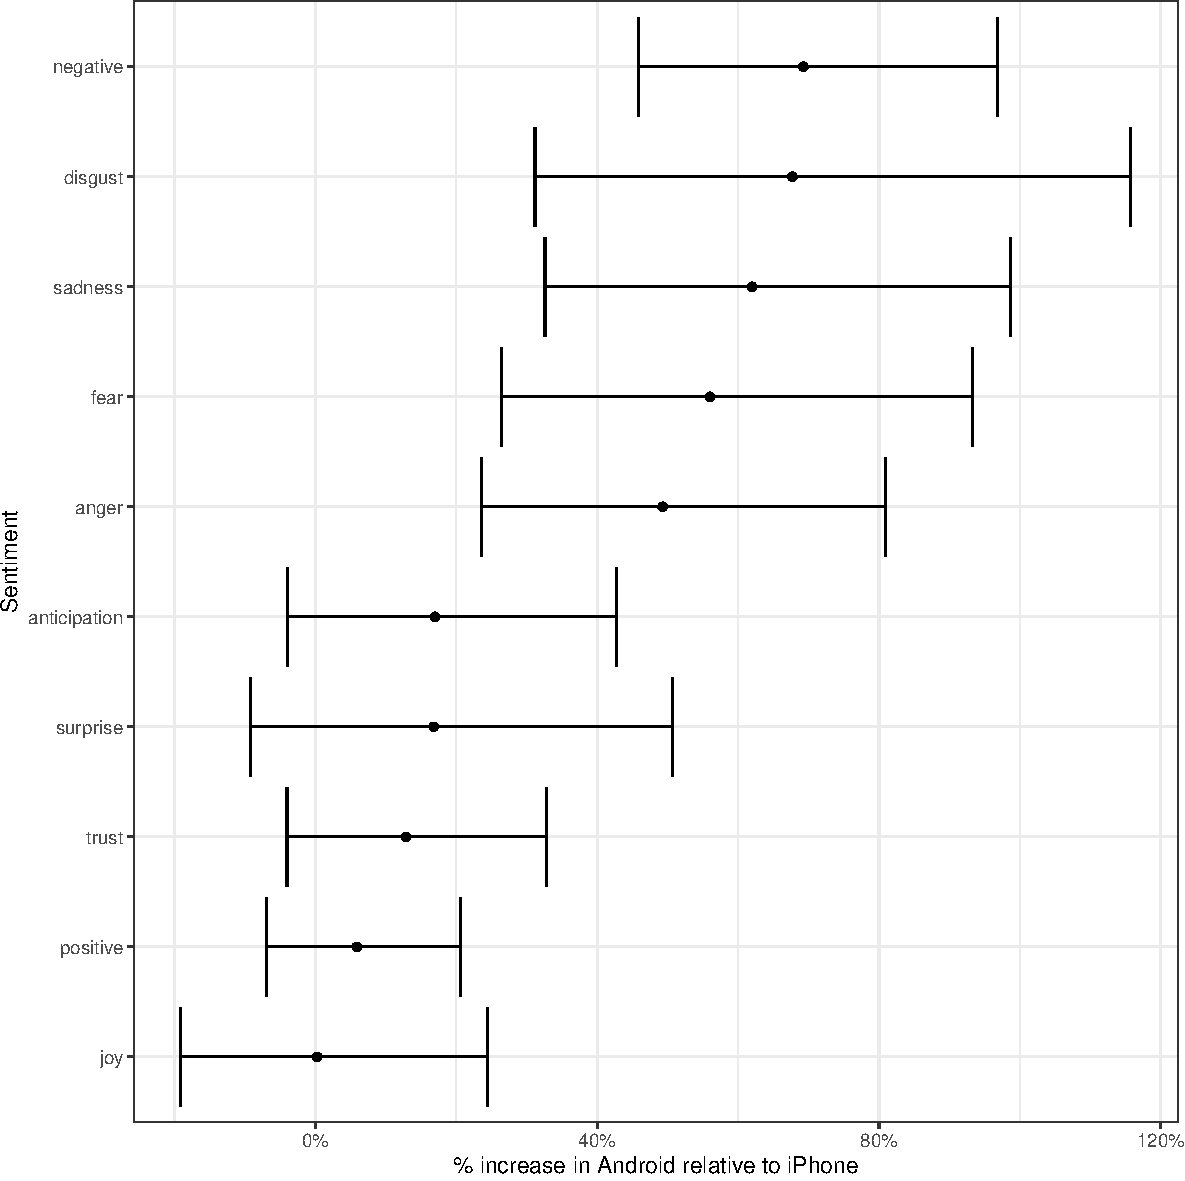
\includegraphics{Live_Demo2_files/figure-latex/unnamed-chunk-7-1} \end{center}

\end{CodeChunk}

Thus, Trump's Android account uses about 40-80\% more words related to
\textbf{disgust}, \textbf{sadness}, \textbf{fear}, \textbf{anger}, and
other ``negative'' sentiments than the iPhone account does. (The
positive emotions weren't different to a statistically significant
extent).

We're especially interested in which words drove this different in
sentiment. Let's consider the words with the largest changes within each
category:

\begin{CodeChunk}


\begin{center}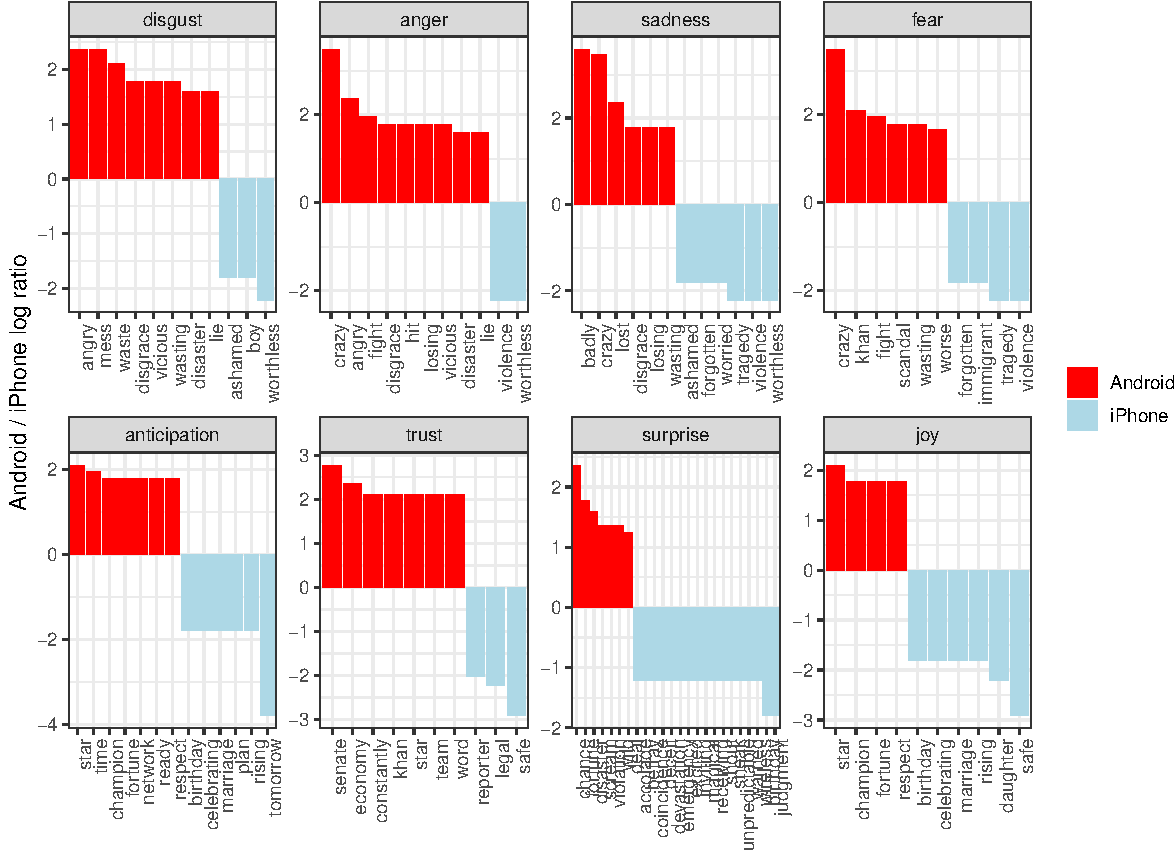
\includegraphics{Live_Demo2_files/figure-latex/unnamed-chunk-8-1} \end{center}

\end{CodeChunk}

This confirms that lots of words annotated as negative sentiments (with
a few exceptions like ``crime'' and ``terrorist'') are more common in
Trump's Android tweets than the campaign's iPhone tweets.

\hypertarget{conclusion-the-ghost-in-the-political-machine}{%
\subsubsection{Conclusion: the ghost in the political
machine}\label{conclusion-the-ghost-in-the-political-machine}}

I was fascinated by the recent
\href{http://www.newyorker.com/magazine/2016/07/25/donald-trumps-ghostwriter-tells-all}{New
Yorker article} about Tony Schwartz, Trump's ghostwriter for The Art of
the Deal. Of particular interest was how Schwartz imitated Trump's voice
and philosophy:

In his journal, Schwartz describes the process of trying to make Trump's
voice palatable in the book. It was kind of ``a trick,'' he writes, to
mimic Trump's blunt, staccato, no-apologies delivery while making him
seem almost boyishly appealing\ldots. Looking back at the text now,
Schwartz says, ``I created a character far more winning than Trump
actually is.''

Like any journalism, data journalism is ultimately about human interest,
and there's one human I'm interested in: who is writing these iPhone
tweets?

The majority of the tweets from the iPhone are fairly benign
declarations. But consider cases like these, both posted from an iPhone:

These tweets certainly sound like the Trump we all know. Maybe our above
analysis isn't complete: maybe Trump has sometimes, however rarely,
tweeted from an iPhone (perhaps dictating, or just using it when his own
battery ran out). But what if our hypothesis is right, and these weren't
authored by the candidate- just someone trying their best to sound like
him?

Or what about tweets like this (also iPhone), which defend Trump's
slogan- but doesn't really sound like something he'd write?

A lot has been written about Trump's mental state. But I'd really rather
get inside the head of this anonymous staffer, whose job is to imitate
Trump's unique cadence (``Very sad!''), or to put a positive spin on it,
to millions of followers. Are they a true believer, or just a cog in a
political machine, mixing whatever mainstream appeal they can into the
\citet{realDonaldTrump} concoction? Like Tony Schwartz, will they one
day regret their involvement?



\end{document}
